The classical PSHA-based damage calculator convolves through numerical
integration, the damage state fragility functions for an asset with the
seismic hazard curve at the location of the asset. The main results of this
calculator are damage distribution statistics for each asset, which describe
the expected fraction of buildings in each damage state. Furthermore, a
probabilistic collapse map can be extracted giving the probability of collapse
for each asset within the specified time period. Damage distribution
aggregated by taxonomy or of the total portfolio (considering all assets in
the exposure model) can not be extracted using this calculator, as the spatial
correlation of the ground motion residuals is not taken into consideration.
The input and output files involved in this calculator are presented in
Figure~\ref{fig:io-structure-classical-damage}.

\begin{figure}[ht]
\centering
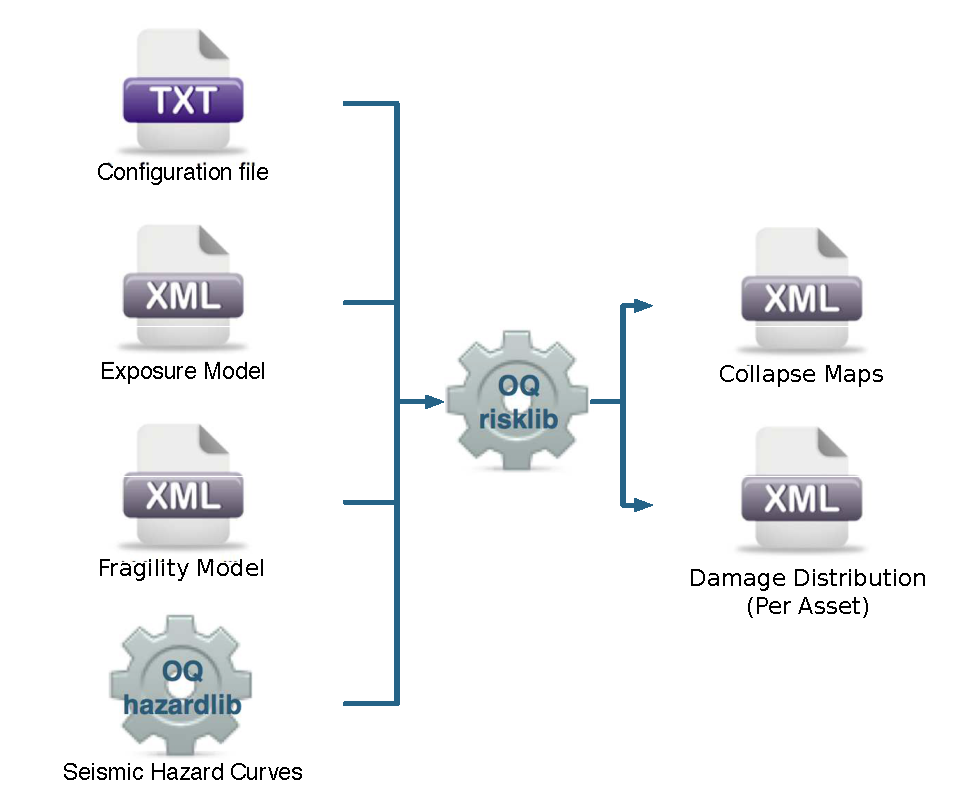
\includegraphics[width=9cm,height=7cm]{figures/risk/io-structure-classical-damage.pdf}
\caption{Classical PSHA-based Damage Calculator input/output structure.}
\label{fig:io-structure-classical-damage}
\end{figure}